
\documentclass[12pt]{article}
\usepackage{geometry} % see geometry.pdf on how to lay out the page. There's lots.
\geometry{a4paper} % or letter or a5paper or ... etc
\usepackage{bm} % see geometry.pdf on how to lay out the page. There's lots.
\usepackage{amsmath}
\usepackage{graphicx}
\usepackage{subcaption}
\usepackage[round]{natbib}
% \geometry{landscape} % rotated page geometry

% See the ``Article customise'' template for come common customisations

\title{Selective constraints on global plankton dispersal}
\author{B.A. Ward, B.B. Cael, C.R. Young and S. Collins}
\date{} % delete this line to display the current date

%%% BEGIN DOCUMENT
\begin{document}
 

\maketitle


Ecotypes - adapted to different environments - but also many more genotypes.

How evolutionarily stable are these genotypes? Do genetic differences represent stable niche separation?

Observations (Kashtan 2014) suggest very hundreds of subpopulations with millions of years genetic dispersal - hence ecologically meaningful.

Clear(?) succession of genetically distinct subpopulations through time

Key question is how much gene flow between environments/niches???




\textit{``Everything is everywhere, but the environment selects''} \citep{BaasBecking:1934}. \citep[Also Beijerinck: one particular species of bacteria found anywhere on Earth, provided environmental requirements are met...][]{Fenchel:2004} ). Oceanic plankton are sufficiently connected such that all species have the potential to colonise all regions. The community that we see in each location is thus determined by ecological selection. 

\citet{Fenchel:2004}: argue that among small organisms ($<$ 1 mm), this connectivity is facilitated by huge population sizes. At local scale, diversity of small species exceeds that of larger species, but at the global scale, diversity of larger species is greater, driven by endemic differences not seen in smaller organisms. 



\citet{Rossberg:2013}: ``Are there any species smaller than 1 mm?'' [Showed empirical trends and used population model. Need to read again!]


Lagrangian studies have been equivocal. \citet{Hellweger:2014} used an agent-based model to estimate the dispersal and mutation of 100,000 `super-individuals'. They found that realistic rates of mutation were enough to sustain several biogeographic provinces, each with a distinct genetic signature, even in the face of realistic ocean mixing. Genotypes found within these provinces were not distributed globally, which they suggest is in conflict with the notion that “everything is everywhere”. However, it seems likely that the model overestimates the rate at which local diversity is lost by genetic drift \citep[i.e. coalescence??][]{Kingman:1982}, because the modelled population size ($10^{5}$ agents) is so small relative to the true population size ($\sim10^{27}$). [Fixation expected in 273 years, rather than $\sim10^{24}$ years].

\citet{Jonsson:2016} used a (biologically inert) particle tracking model in combination with Dijkstra's `shortest-path algorithm' \citet[][]{Dijkstra:1959} to show that pathways exist to connect the global ocean on timescales of a decade or less. Even though some of the shortest paths are quite unlikely, the huge size of planktonic populations is again invoked to suggest that the pathways should be followed by at least some individuals.  \citet{Jonsson:2016} do not account explicitly for population size, and it remains to be seen how population size and biogeography might affect the predicted patterns of connectivity.


Stochastic approach that accounts for the enormous and variable size of plankton (meta) populations, the potential for stochastic dispersal, and/or a representation of natural selection.

\section{Methods}


\begin{figure}[htp!]
\centering
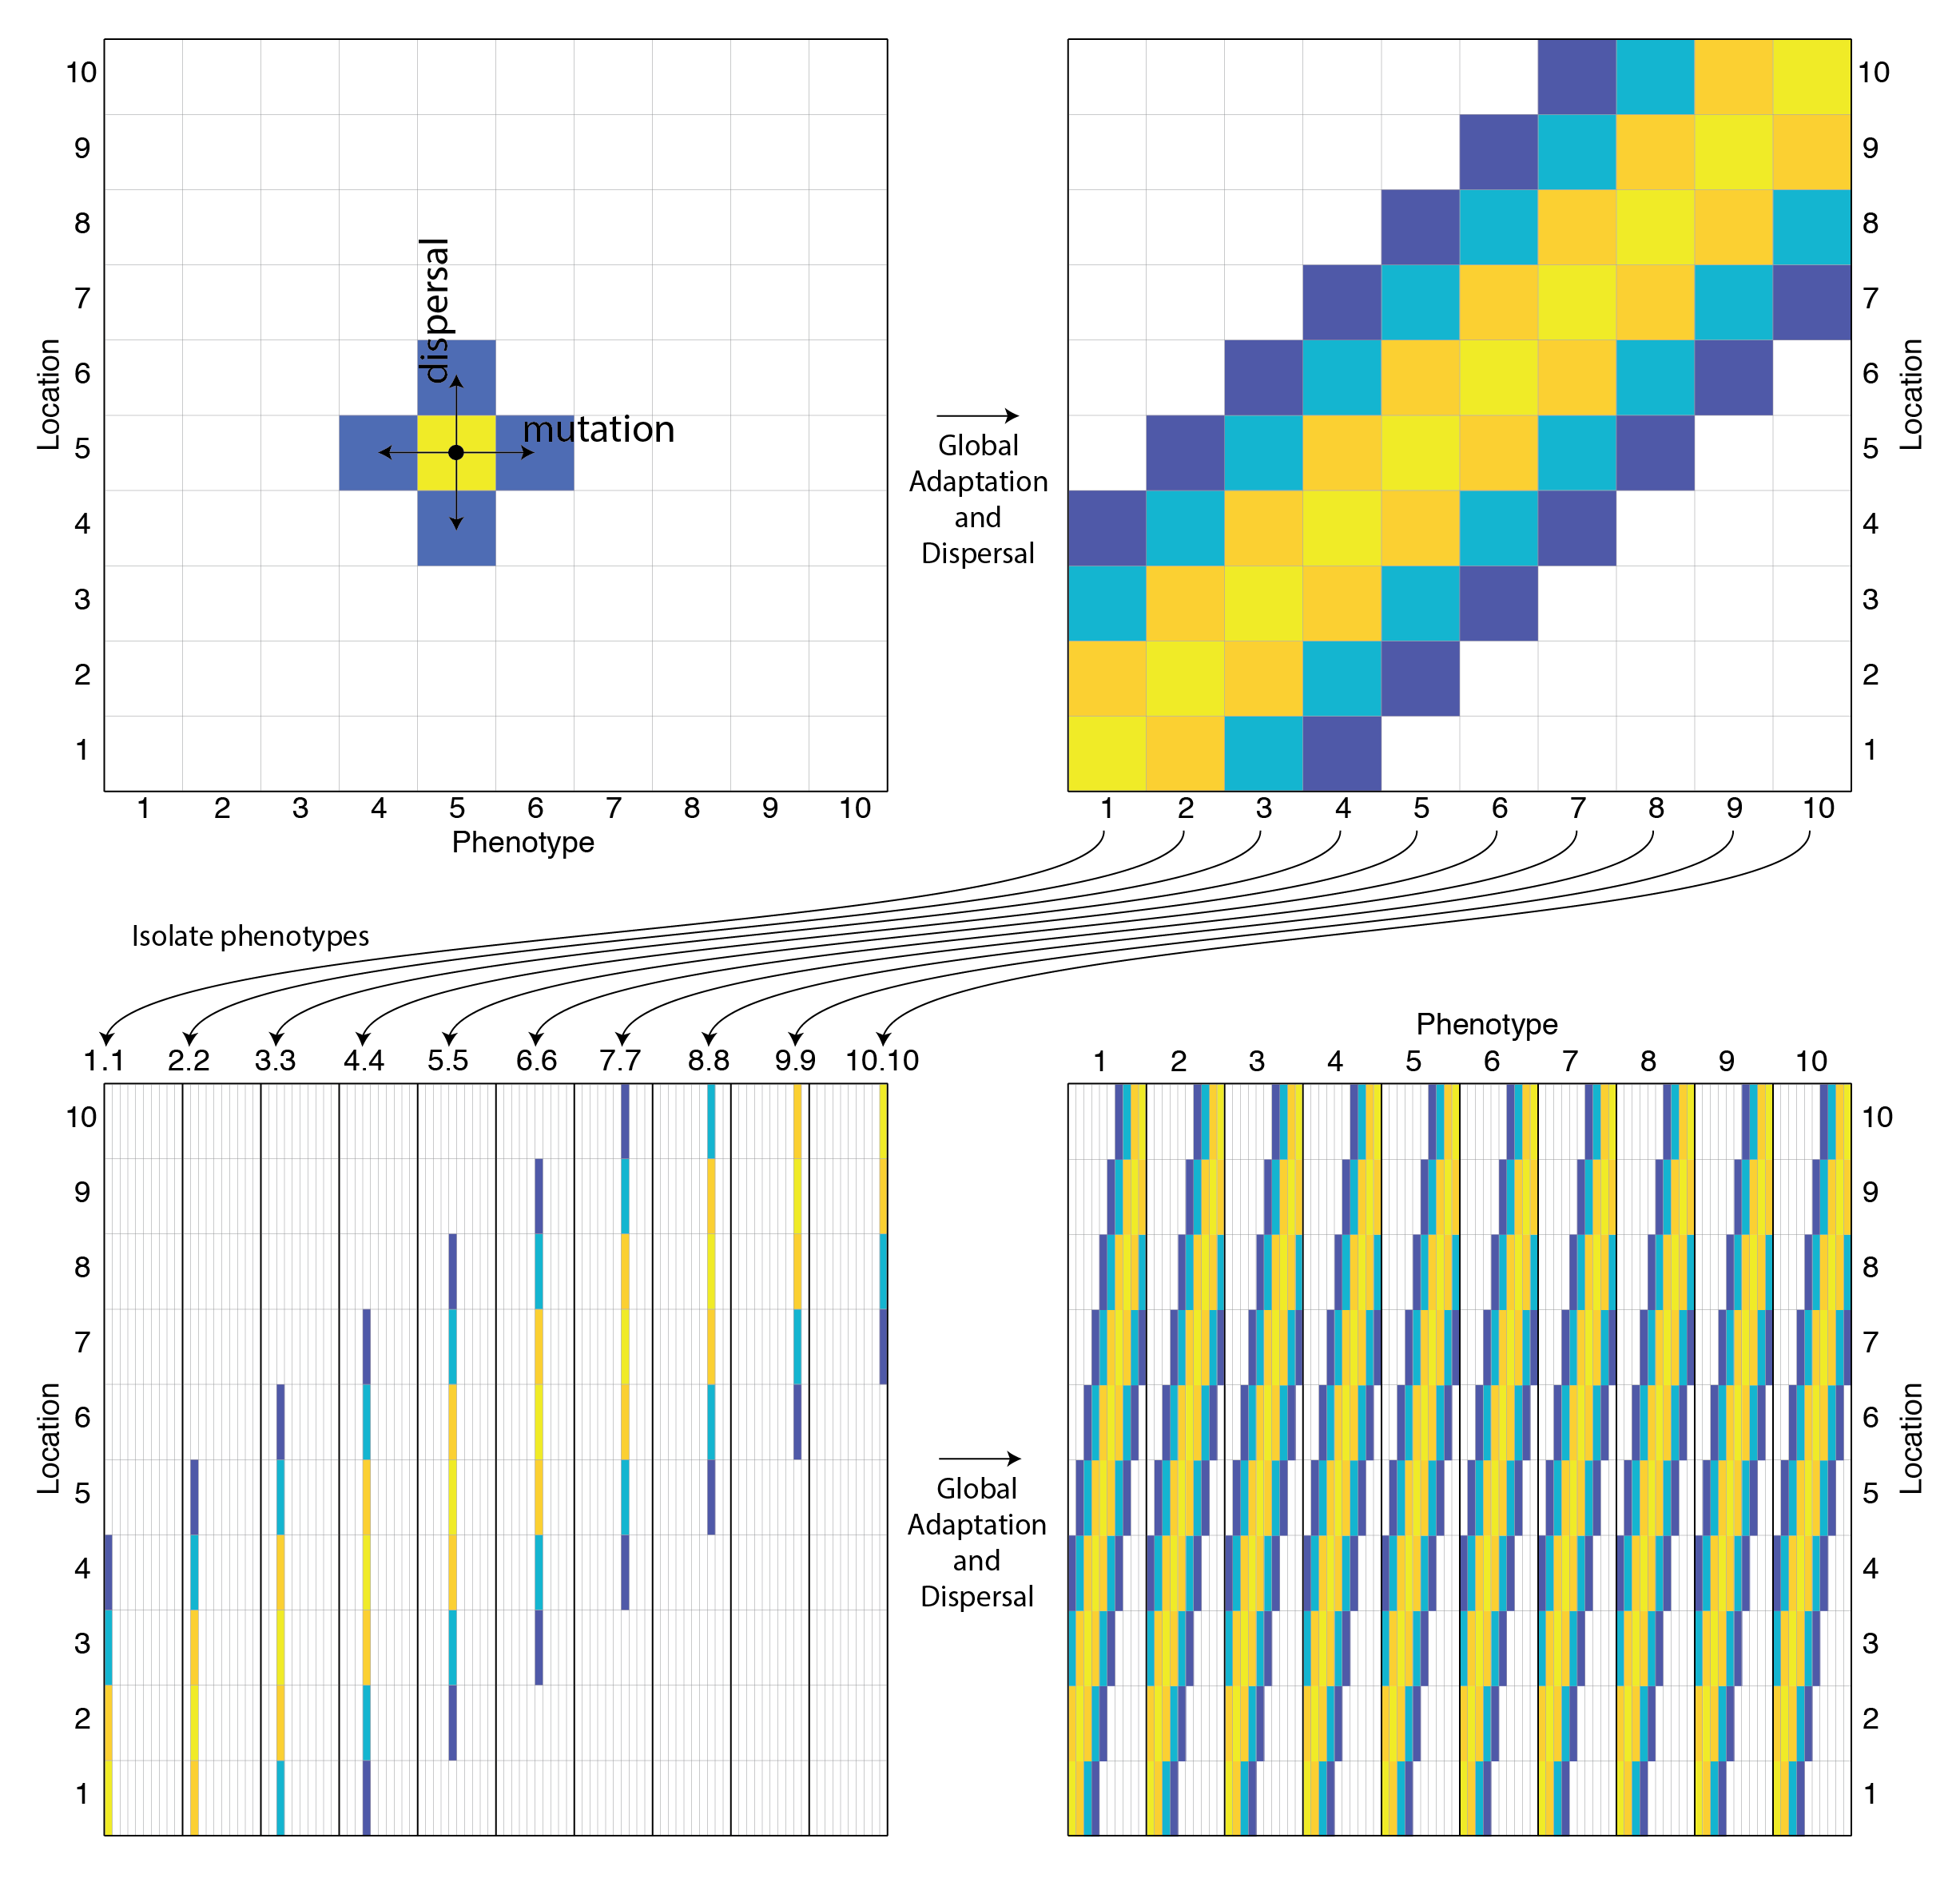
\includegraphics[width=0.8\linewidth]{../Figures/Schematic.png}
\caption{}
\label{Schematic}
\end{figure}


\begin{figure}[htp!]
%%
\begin{subfigure}{0.5\textwidth}
\includegraphics[width=1\linewidth]{../Output/neutral_stochastic_static_GUD_X01_surface_transport/connection_times_map.png}
\end{subfigure}
%%
\begin{subfigure}{0.5\textwidth}
\includegraphics[width=1\linewidth]{../Output/neutral_stochastic_static_GUD_X01_weighted_transport/connection_times_map.png}
\end{subfigure}
%%
\begin{subfigure}{0.5\textwidth}
\includegraphics[width=1\linewidth]{../Output/neutral_stochastic_static_GUD_X17_weighted_transport/connection_times_map.png}
\end{subfigure}
%%
\begin{subfigure}{0.5\textwidth}
\includegraphics[width=1\linewidth]{../Output/neutral_stochastic_static_GUD_X17_weighted_transport/connection_times_map.png}
\end{subfigure}
%%
\caption{}
\label{Schematic}
\end{figure}


\begin{figure}[htp!]
%%
\begin{subfigure}{0.5\textwidth}
\includegraphics[width=1\linewidth]{../Output/neutral_stochastic_static_GUD_X01_weighted_transport/connection_matrix.png}
\end{subfigure}
%%
\begin{subfigure}{0.5\textwidth}
\includegraphics[width=1\linewidth]{../Output/neutral_stochastic_static_GUD_X17_weighted_transport/connection_matrix.png}
\end{subfigure}
%%
\caption{}
\label{Schematic}
\end{figure}



\subsection{Plankton as passive tracers}

We consider the global abundance of a plankton population with $K$ genotypes within $J$ spatial boxes of an ocean general circulation model (GCM). Local cell abundances within each genotype are thus represented in the $[J\times K]$ population matrix.

Plankton cells are transported between grid boxes using a $[J\times J]$ oceanic `transport matrix' $\mathbf{A}$ that describes the volume transport attributable to advection, diffusion and parameterised sub-grid-scale processes in the GCM \cite{Khatiwala:2005}. This transport can be written as a linear matrix equation \cite{Khatiwala:2005}, with the form

\begin{equation}
\frac{d\mathbf{x}}{dt} = \mathbf{A}\mathbf{X}
\end{equation}

Here $\mathbf{X}$ is the $[J\times K]$ matrix of genotype frequencies in each grid box of the GCM. Each element of the transport matrix $\mathbf{A}$ describes the mass flux between source boxes (columns) and recipient boxes (rows). The diagonal elements of the transport matrix should always be nonpositive ($<=0$), as they describe the mass flux out of the source box to other (nearby) boxes. Similarly, the off-diagonal elements should always be nonnegative ($>=0$), as they describe the mass flux into the recipient box from other nearby boxes. 

This gives the following explicit form of the linear matrix equation

\begin{equation}
\label{ }
\mathbf{X}_{t+1}=\mathbf{D}\mathbf{X}_{t}
\end{equation}

%\subsection{Shortest path connectivity}
%Given that $\mathbf{D}$ describes the volume-specific rate of water flux among each of the GCM grid boxes, then $\mathbf{T}=[\mathbf{D}>0]^{-1}$ is the expected waiting time for an individual water molecule (or particle) to pass from one grid box to the next (assuming each grid cell is perfectly mixed). We can then use Dijkstra's shortest path algorithm to calculate the shortest path direct between any two points in the ocean, with path length defined as the sum of expected waiting times along the path. We can also calculate the probability of a single particle directly following the shortest path, as the product of each element in $\mathbf{D}$ corresponding to that path.

%[dist,path,pred] = graphshortestpath(weighted',s,t);\\
%isnk=path(2:end);\\
%isrc=path(1:end-1);\\
%P=sum(log10(B(sub2ind(size(B),isnk,isrc))));


\subsection{Stochastic dispersal}

Each grid box supports a predefined carrying capacity of $\mathbf{n}$ individuals. Under strict neutrality, the number of individuals $\mathbf{X}$ surviving at each generation is drawn randomly from the local population (after oceanic transport) with probability equal to the local genotype frequency ($\mathbf{p} = \mathbf{X} \mathbf{n}^{-1}$). Under these assumptions, the expected population size in each generation is given by the multinomial distribution, 

\begin{equation}
\label{eqn:mnml}
\mathbf{X}\sim\mathcal{M}(\mathbf{n},\mathbf{p})
\end{equation}

For large $\mathbf{N}$, equation~\ref{eqn:mnml} is reasonably approximated by a normal distribution.

\begin{equation}
\mathbf{X}\approx\mathcal{N}(\boldsymbol{\mu},\boldsymbol{\sigma})
\end{equation}

with $\boldsymbol{\mu}=\mathbf{n}\circ\mathbf{p}$ and $\boldsymbol{\sigma}=\mathbf{n}\circ\mathbf{p}\circ(1-\mathbf{p})$. (Here the `$\circ$' symbol denotes element-wise multiplication.)

\subsection{Connectivity}

We used the population model to estimate the global dispersal of 341 genotypes, each initialised at unique ``seed locations'' that were distributed approximately evenly around the surface ocean. We also included one additional tracer representing a globally resident species, with a genotype frequency of $\mathbf{p} = 0$ at all seed locations, and 1 throughout the rest of the surface grid.

We estimated minimum connectivity times by integrating the model forward from these initial conditions, noting the time at which each genotype first appeared in each grid cell. 


\subsection{Selection}

Selection can be further incorporated through the selection vector $\mathbf{s}$, that assigns each population in $\mathbf{X}$ a relative fitness of $1+\mathbf{s}$.

\begin{equation}
\label{ }
\mathbf{p} = \frac{\mathbf{\tilde{p}} \circ (1+\mathbf{s}) } {\mathbf{\tilde{p}} \circ (1+\mathbf{s}) + 1 -\mathbf{\tilde{p}}}
\end{equation}

\textbf{[NOT YET GENERALISED FOR MULTINOMIAL]}


%If we model just two genotypes, the expected population size in each generation of the first genotype is given by the binomial distribution, 
%\begin{equation}
%\label{eqn:mnml}
%\mathbf{X_1}\sim\mathcal{B}(\mathbf{n},\mathbf{p_1})
%\end{equation}
%The binomial distribution is also reasonably approximated by a normal distribution for large $\mathbf{N}$. The expected population size of each genotype is then simply $\mathbf{X_2} = \mathbf{N}-\mathbf{X_1}$.


Thermal niche. Seed with n plankton types, each adjusted to a different optimal temperature. How connected are these phenotypes? How does the connectivity depend on population size? on the shape of the thermal niche? Do results compare well with Thomas 2012 or Righetti 2019?

\begin{equation}
\gamma_T = a e^{bT} e^{\Big(-\big(\frac{2(T-z)}{w}\big)^2\Big)}
\end{equation}


\section{Results}

\subsection{Timescales of dispersal}

Seed subset of ocean regions with one tracer each. Examine time until globally distributed. Dispersal potential increases with local population size.


\begin{figure}[htp!]

\caption{Left-hand side: global abundance distribution of prochlorococcus (top) and diatoms (bottom). Right-hand side: timescales of ocean connectivity for the same two groups. Background colour: shortest timescales over which particles from 95\% of the seed locations (indicated by dots) are expected to have arrived at each point (i.e. immigration timescales). Dots: timescales over which particles from that seed location are expected to have arrived at 95\% of the ocean surface (i.e. emigration timescales).}
\label{connectivity_90_prctile}
\end{figure}



\subsection{Spatial clustering by timescales of connectivity}


\begin{figure}[htp!]

\caption{Pairwise global minimum connectivity and clustering. Upper panel: matrix of the connectivity times between seed locations. Columns of the matrix correspond to source locations (such that row values represent emigration timescales), while rows correspond to target locations (such that column values represent immigration timescales). Lower panel: Clustering of the seed locations on the basis of the average of the immigration and emigration timescales between each location. Coloured boxes in the upper panel indicate clusters defined by the average timescales of connectivity (as shown in the lower panel).}
\label{connectivity_matrices}
\end{figure}



\begin{figure}[htp!]

\caption{Spatial distribution of the 15 connectivity clusters. Colours and numbers correspond to those used in Figure~\ref{connectivity_matrices}.}
\label{Connectivity_maps}
\end{figure}

\begin{figure}[htp!]

\caption{Number of globally unconnected points through time}
\label{Connectivity_maps}
\end{figure}






%\subsection{Expected shortest path connectivity}
%The shortest path between the Arctic Ocean and Weddel Sea in the ECCO GCM traverses only 500 grid boxes. It could, in theory, be completed in under two years. However, probability of a single particle following all 500 required steps in sequence is effectively zero (actually 10$^{-662}$). By accounting for the expected waiting time between grid cells, we can come up with a more realistic estimate for the expected journey time of 41 years. This is the average time taken for any particles that do follow the shortest path, accounting for time spent waiting in each grid box.
%Applying the transport matrix until all shortest paths have been followed...
%\begin{equation}
%\label{ }
%\mathbf{B} = \mathbf{A}^n
%\end{equation}




\clearpage 

\appendix

\section{Appendix}

\subsection{Mass conservation correction}

Numerical constraints within the GCM mean that some off-diagonal elements may be negative. To remove these artefacts, negative fluxes out of a box are converted to positive fluxes into the box. If we first define the matrix of negative off-diagonal elements as follows,

\begin{equation}
N_{i,j} = 
\begin{cases}
0 		& \text{if $i=j$ or $A_{i,j}\ge 0$}\\
A_{i,j} 	& \text{if $i\ne j$ and $A_{i,j}<0 $}
\end{cases}
\end{equation}

We first move the off-diagonal negatives to their transpose, changing the sign.

\begin{equation}
\mathbf{B} = \mathbf{A} - \mathbf{N} + ( - \mathbf{N}^\top)
\end{equation}

To conserve mass, changes in the off-diagonals must be compensated by an equivalent change on the diagonals. This is achieved by adding both the row and column sums of the negative off-diagonals to the diagonal. 

\begin{equation}
C_{i i} = B_{i i} + \sum_{j=1}^J N_{i,j} + \sum_{j=1}^J N_{j,i} \text{ (for all $i$)}
\end{equation}

The resultant matrix is positive-definite on the off-diagonals, and conserves mass.

Finally, the transport matrix is converted from a volume flux per time (m$^3$~d$^{-1}$) to a unitless operator; first dividing through by the volume of the recipient cells ($\mathbf{v}$), then multiplying by the selected time step ($\Delta t$), and adding the identity matrix ($\mathbf{I}$).

\begin{equation}
\mathbf{D} = \frac{\mathbf{C}}{\mathbf{v}} \times \Delta t + \mathbf{I}
\end{equation}

\subsection{Seed locations}

Seed locations were identified by iteratively projecting a subdivided rectangular grid onto the surface of a sphere. Surface ocean coordinates from the GCM grid were then mapped onto these points (by shortest euclidean distance in cartesian coordinates). Finally, the 341 unique coordinates were mapped back to their nearest point on the GCM grid. The model was initialised with one tracer for each of these points, with a genotype frequency of $\mathbf{p} = 1$ at the seed location, and zero everywhere else. 


\bibliography{/Users/baw103/GoogleDrive/biblio1}
\bibliographystyle{/Users/baw103/Latex/elsart-harv.bst}
\end{document}













